\chapter{Mener une action d'amélioration d'un atelier de travail avec  Audit, les outils lean 4.0}\label{chap2}

\lhead{Chapitre II: Audit et DMAIC }
\dominitoc 
\rhead{\thepage}
\begin{spacing}{2}
\minitoc
\end{spacing}
\section{Introduction}
\label{chap2:intro}

Ce deuxième chapitre présente de manière structurée et systématique la démarche méthodologique employée pour analyser et améliorer les performances de l'atelier de coupe. L'architecture de ce chapitre s'organise en deux parties complémentaires et interdépendantes.

La première partie expose le \textbf{diagnostic de maturité digitale} de l'atelier de coupe réalisé au travers d'un \textbf{audit approfondi} et structuré, fondé sur le référentiel international \textbf{IMPULS} (Industrie 4.0 Maturity Index) spécifiquement conçu pour l'évaluation de la maturité digitale industrielle. Cet audit méthodologique permet d'évaluer de manière objective et quantifiée le niveau de digitalisation actuel de l'atelier, et d'identifier de manière priorisée les axes stratégiques d'amélioration en cohérence avec les standards de l'Industrie 4.0.

La seconde partie détaille l'application rigoureuse et systématique de la \textbf{méthodologie DMAIC} (\textit{Define, Measure, Analyze, Improve, Control}), issue du référentiel \textbf{Lean Six Sigma}, mise en œuvre dans le cadre d'une \textbf{action d'amélioration Lean 4.0} visant a identifier de manière structurée les dysfonctionnements opérationnels de l'atelier de coupe, a quantifier leurs impacts, a analyser leurs causes racines, et a proposer des solutions d'amélioration fondées sur des données objectives.

L'objectif principal de cette démarche méthodologique combinée est d'établir une base solide, rigoureuse et fondée sur des preuves empiriques pour la conception et le développement de \textbf{solutions digitales intelligentes}, en s'appuyant a la fois sur une \textbf{évaluation objective du niveau de maturité digitale} et sur une \textbf{analyse quantitative approfondie des performances actuelles} de l'atelier.

\section{Partie I : Audit de maturité digitale}

\subsection{Introduction a l'audit IMPULS}

Dans un contexte de transformation numérique croissante, il est essentiel d'\textbf{évaluer le niveau de maturité digitale} des différents services de production. L'audit de maturité digitale permet d'identifier les forces, les faiblesses et les opportunités d'évolution vers les standards de l'Industrie 4.0.

\subsection{Objectifs de l'audit}

\begin{itemize}
\item Évaluer le niveau d'intégration des technologies numériques dans l'atelier de coupe
\item Identifier les axes d'amélioration en lien avec l'excellence opérationnelle et l'Industrie 4.0
\item Préparer un plan d'action de transformation digitale adapté a la réalité terrain
\end{itemize}



\subsection{Phase Innover : Propositions d'€™amélioration}

\subsubsection{Constat principal}

L'€™analyse de la phase \textit{Analyze} a révélé plusieurs dysfonctionnements limitant la performance de l'€™atelier de coupe, notamment une \textbf{saturation rapide des tables de matelassage} due a l'€™absence de système de planification et de suivi en temps réel.

Ces contraintes se traduisent par :
\begin{itemize}
  \item Une \textbf{indisponibilité fréquente} des tables lors des pics d'€™activité ;
  \item Des \textbf{conflits de planification} entre opérateurs, dus a un manque de visibilité globale sur les ressources ;
  \item L'€™absence d'€™un \textbf{outil numérique} permettant de synchroniser le planning avec l'€™état réel des tables.
\end{itemize}

Ces constats soulignent la nécessité d'€™un \textbf{pilotage intelligent des ressources}, s'€™inscrivant pleinement dans la logique de l'€™Industrie 4.0, ou la digitalisation et l'€™automatisation des processus permettent de renforcer la réactivité et l'€™efficacité opérationnelle.

\subsubsection{Proposition : Algorithme intelligent de gestion des tables de matelassage}

Afin d'€™optimiser la planification et l'€™utilisation des ressources physiques de l'€™atelier, nous proposons un \textbf{algorithme de gestion dynamique} des tables de matelassage. Cet outil vise a offrir une \textbf{visualisation en temps réel} de la disponibilité des tables, tout en anticipant les conflits d'€™utilisation.

\paragraph{Principe de fonctionnement}
Chaque table est identifiée par un code unique (T1, T2, \dots, T6). Le système compare en continu l'€™heure actuelle avec le planning de matelassage. Il met automatiquement a jour le statut de chaque table selon trois états possibles : \textit{Occupée} (en cours d'€™utilisation), \textit{Réservée} (prévue pour une opération a venir) et \textit{Disponible} (libre pour un nouveau matelas).

\paragraph{Pseudocode de l'€™algorithme}
\begin{verbatim}
Entrées :
  Tables = {T1, T2, …, T6}
  Planning (heure début, durée prévue)
  Heure actuelle = H

Pour chaque table T[i] :
  Si (H >= heure début[i] ET H < heure fin prévue[i]) :
      Statut[T[i]] = "Occupée"
  Sinon si (H < heure début[i]) :
      Statut[T[i]] = "Réservée"
  Sinon :
      Statut[T[i]] = "Disponible"

Afficher le statut de chaque table
\end{verbatim}

\subsubsection{Application pratique}
L'€™algorithme peut etre déployé sous plusieurs formes :
\begin{itemize}
  \item \textbf{Une feuille Excel automatisée}, avec macros et mise a jour minute par minute ;
  \item \textbf{Une interface web locale}, connectée aux données de production et accessible depuis le poste du chef d'€™atelier.
\end{itemize}
Ce système permet :
\begin{itemize}
  \item de \textbf{visualiser en temps réel} la disponibilité de chaque table ;
  \item d'€™\textbf{éviter les conflits} ou chevauchements de planning ;
  \item d'€™\textbf{améliorer la fluidité} du flux de travail entre préparation, matelassage et coupe.
\end{itemize}

\begin{table}[H]
\centering
\caption{Exemple de statut temps réel}
\begin{adjustbox}{max width=\textwidth}
\begin{tabular}{|l|l|l|}
\hline
\textbf{Table} & \textbf{Heure actuelle} & \textbf{Statut} \\
\hline
T1 & 09:00 & Occupée (jusqu'€™a 09:30) \\
\hline
T2 & 09:00 & Disponible \\
\hline
T3 & 09:00 & Occupée (jusqu'€™a 09:45) \\
\hline
\end{tabular}
\end{adjustbox}
\end{table}

\subsubsection{Bénéfices attendus}
L'€™intégration de cet algorithme dans le système de gestion de production offre plusieurs avantages :
\begin{itemize}
  \item \textbf{Réduction du temps d'€™attente} entre les opérations de coupe ;
  \item \textbf{Optimisation de l'€™utilisation des ressources existantes} sans investissement matériel supplémentaire ;
  \item \textbf{Amélioration de la coordination} entre opérateurs et planificateurs ;
  \item \textbf{Digitalisation partielle du pilotage de production}, contribuant a la transition vers une \textbf{usine connectée}.
\end{itemize}
Ainsi, cette solution constitue une première étape vers la \textbf{transformation numérique} de l'€™atelier, en s'€™inscrivant dans une démarche \textit{Lean 4.0} conciliant \textbf{amélioration continue} et \textbf{technologies intelligentes}.

\subsection{Méthodologie d'évaluation}

\subsubsection{Choix du questionnaire IMPULS}

Le questionnaire \textbf{IMPULS – Industrie 4.0 Readiness} \cite{lichtblau2015industrie} a été choisi pour sa pertinence dans l'analyse de la maturité digitale industrielle \cite{xu2018industry, kagermann2013recommendations}. Il couvre les thématiques suivantes :
\begin{itemize}
   \item Efficacité des processus
   \item Automatisation, innovation et intégration numérique
   \item Gestion des performances et des flux
   \item Amélioration continue et flexibilité
\end{itemize}

\subsubsection{Mode de diffusion}

Le questionnaire a été administré en ligne via Google Forms, avec un accompagnement en présentiel pour aider les répondants a bien comprendre chaque question technique.

\subsubsection{Cible de l'enquete}

L'enquete a ciblé \textbf{11 personnes clés} de l'atelier de coupe, incluant :
\begin{itemize}
  \item Chef d'atelier
  \item Agents d'ordonnancement/planification
  \item Opérateurs machine
  \item Responsables qualité coupe
  \item Responsable maintenance
\end{itemize}
Ces profils ont été choisis en fonction de leur connaissance du fonctionnement réel
de l'€™atelier et de leur implication dans les processus numériques ou manuels actuels.
\subsection{Déroulement de l'€™enquete}
\begin{itemize}
  \item  \textbf  Préparation : création du formulaire Google Forms (Figure \ref{form}), adaptation des questions a l'€™environnement Bacovet.

  \item  \textbf  Lancement : envoi du lien aux personnes concernées, accompagnement en face a face sur place.

  \item  \textbf  Assistance : chaque répondant a été guidé par l'€™auteur du projet pour expliciter les critères du questionnaire.

  \item  \textbf  Collecte et consolidation : les réponses ont été collectées automatiquement, puis exploitées pour l'€™analyse.(Les Figures \ref{20};\ref{22})
 \end{itemize}
 \begin{figure}[H]
  \centering
  \begin{minipage}[b]{0.30\textwidth}
    \centering
    \includegraphics[width=\textwidth]{Chapitre2/images/21.jpg}
    \caption{Formulaire Google Forms}
    \label{form}
  \end{minipage}
  \hfill
  \begin{minipage}[b]{0.30\textwidth}
    \centering
    \includegraphics[width=\textwidth]{Chapitre2/images/20.jpg}
    \caption{Diagramme circulaire (Pie chart)}
    \label{20}
  \end{minipage}
  \hfill
  \begin{minipage}[b]{0.30\textwidth}
    \centering
    \includegraphics[width=\textwidth]{Chapitre2/images/22.jpg}
    \caption{Histogramme / Diagramme en barres (Bar chart)}
    \label{22}
  \end{minipage}
\end{figure}


\section{Résultats de l'évaluation de la maturité digitale}
\subsection{Méthodologie d'évaluation}

\begin{methodBox}
L'évaluation de la maturité digitale de l'atelier de coupe a été réalisée a l'aide du questionnaire \textbf{IMPULS}, un outil de diagnostic développé par l'Association Allemande de l'Industrie (VDMA) pour mesurer l'état d'avancement des entreprises dans l'adoption des principes de l'Industrie 4.0.
\end{methodBox}

L'€™évaluation de la maturité digitale a été effectuée a l'€™aide d'€™un calculateur basé sur les retours de 11 répondants. Chaque critère a été noté selon trois niveaux d'€™implémentation : « Non », « Partiellement », et « Oui », permettant de générer un score global par critère .
\subsection{Détail des scores par critère}

\begin{figure}[p]
\centering
\includegraphics[angle=90,width=1.3\textheight,height=1.3\textwidth,keepaspectratio]{Chapitre2/images/IMG_20250614_141256_509.jpg}
\caption{Fiche d'enregistrement (modèle Rim)}
\label{chpp3}
\end{figure}

\begin{figure}[p]
\centering
\includegraphics[angle=90,width=1.3\textheight,height=1.3\textwidth,keepaspectratio]{Chapitre2/images/IMG_20250614_141303_456.jpg}
\caption{Fiche d'enregistrement (modèle Leotard 500g pink)}
\label{chp3}
\end{figure}

\end{itemize}

\paragraph{Analyse du déroulement de coupe (extrait documentaire)}

Afin de compléter la collecte terrain, une \textbf{analyse documentaire} a été réalisée a partir du fichier \textit{analyse deroulement COUPE}. Cette source décrit pas-a-pas le déroulement d'articles en coupe et sert de support a la validation des séquences observées et des points de mesure.

\paragraph{Aperçu (intégration directe du PDF)}
À défaut de captures déja extraites, les pages clés du document sont intégrées ci-dessous directement depuis le PDF.

\includepdf[pages=1,angle=90,scale=0.85,pagecommand=\thispagestyle{plain}]{Chapitre2/analyse_deroulement_coupe.pdf}

\paragraph{Description synthétique du document}
Le document \textit{analyse deroulement COUPE} présente, sous forme structurée et illustrée, le déroulement réel des opérations dans la salle de coupe. Il décrit successivement les étapes de préparation (CAO, vérification OF et matières), de matelassage (manuel et automatique), de coupe (robotisée et/ou manuelle), puis de départage et vignettage, en précisant pour chaque étape les acteurs impliqués, les supports utilisés, les temps observés, ainsi que les incidents/perturbations relevés (pannes, attentes, changements de priorité, relaxation tissu, etc.).

\paragraph{Objectifs de l'analyse documentaire}
\begin{itemize}
    \item Valider, par triangulation, les séquences opérationnelles observées sur le terrain et celles décrites par les procédures internes.
    \item Identifier les points de contrôle utiles a la mesure (horodatages, transitions d'étapes, variables influentes comme nombre de plis, laize, longueur).
    \item Mettre en évidence les sources récurrentes de variabilité et de perturbation impactant la planification (attentes tables, pannes robot, relaxation doublure, saisies manuelles).
    \item Définir une base de référence fiable pour la modélisation des temps et l'optimisation ultérieure (chapitres Analyse et Amélioration).
\end{itemize}

\paragraph{Principaux enseignements}
\begin{itemize}
    \item Les transitions entre matelassage et coupe constituent un point critique de synchronisation; l'absence de visibilité temps réel génère des attentes et des replanifications.
    \item Le temps de matelassage est fortement corrélé au nombre de plis et aux dimensions du matelas; la variabilité opérateur/machine demeure notable.
    \item Les perturbations majeures recensées (pannes robot, relaxation tissu, changements de priorité) expliquent une part significative des écarts planning.
    \item La traçabilité amont/aval est partielle: des données clés restent saisies manuellement et non consolidées.
\end{itemize}

\paragraph{Limites et précautions}
\begin{itemize}
    \item La documentation se concentre sur des cas représentatifs mais non exhaustifs; elle doit etre complétée par des mesures systématiques et des séries temporelles plus longues.
    \item Certaines informations (délais d'attente, durées anormales) peuvent etre sous-déclarées en l'absence d'instrumentation continue.
\end{itemize}

\paragraph{Conclusion opérationnelle}
Cette analyse documentaire consolide la compréhension du flux réel en salle de coupe et fournit des repères mesurables pour la phase \textbf{Analyser}. Elle justifie la mise en place d'une instrumentation de mesure plus fine, l'amélioration de la visualisation temps réel et l'usage d'un modèle prédictif des temps de matelassage/coupe pour soutenir la planification.

% (Figures dé\end{itemize}placées plus haut, juste après le paragraphe de chronométrage direct)

% Figure supprimée sur demande (anciennement: Fiche d'enregistrement du déroulement de chaque article)

\subsubsection{Description synthétique des processus mesurés}

Les activités mesurées et leurs ordres de grandeur observés sont :
\begin{itemize}
    \item \textbf{Préparation des fichiers CAO} et traçabilité OF : 50 a 60 minutes.
    \item \textbf{Matelassage automatique} (1 table dédiée, chariot automatisé) : 20 a 30 minutes par matelas selon le tissu.
    \item \textbf{Matelassage manuel} (4 tables, 2 opérateurs/table) : 35 a 50 minutes par matelas.
    \item \textbf{Coupe robotisée} (2 robots horizontaux, 5 tables) : 25 a 40 minutes selon la complexité.
    \item \textbf{Départage et ajout de vignettes} (13 opérateurs) : 40 a 60 minutes par lot.
    \item \textbf{Stockage et contrôle qualité} : transfert vers trois zones de stockage (avant/après sérigraphie).
\end{itemize}

\subsubsection{Constats clés de la collecte}

\begin{itemize}
    \item \textbf{Variabilité des temps} par modèle (jusqu'a ±15 min sur matelassage manuel).
    \item \textbf{Perturbations fréquentes} : pannes des robots (notamment robot 2), pannes d'électricité, attente de relaxation tissu (jusqu'a 72h pour la doublure).
    \item \textbf{Communication manuelle} et absence d'outil de visualisation partagée du planning.
\end{itemize}

\subsubsection{Paramètres techniques de l'atelier (référence)}

\begin{table}[H]
\centering
\begin{adjustbox}{max width=\textwidth}
\begin{tabular}{|l|l|}
\hline
\textbf{Élément} & \textbf{Valeur} \\
\hline
Nombre de tables & 6 (dont 1 automatique, 4 manuelles, 1 vide) \\
\hline
Chariot matelasseur automatique & 1 \\
\hline
Robots de coupe & 2 (translation horizontale sur 5 tables) \\
\hline
Effectif sur les tables & 17 opérateurs \\
\hline
Équipe de départage & 13 postes / 13 personnes \\
\hline
Zones de stock & 3 (avant/après sérigraphie) \\
\hline
\end{tabular}
\end{adjustbox}
\caption{Paramètres techniques de l'atelier}


\label{tab:parametres_atelier_phase2}
\end{table}


\subsubsection{Synthèse de la phase de mesure}

La phase \textbf{Mesurer} quantifie les écarts entre le planning théorique et la réalité opérationnelle. Les données montrent l'impact des pannes machines, du manque de visualisation temps réel et de l'absence de remontées automatiques, générant des \textbf{retards non détectés} et une fiabilité de planning dégradée. Ces éléments constituent la base de la phase \textbf{Analyser} qui suit.

\subsection{Phase 3 : Analyze (Analyser)}

\subsubsection{Objectif de la phase Analyse}

La phase \textbf{Analyse} vise a identifier les causes racines des perturbations observées dans la planification de l'atelier de coupe. Elle s'appuie sur les résultats collectés durant la phase de mesure, notamment les données chronométrées, les pannes, et la disponibilité des ressources.

L'objectif est de comprendre pourquoi les délais de matelassage et de coupe varient, et quelles sont les sources principales des retards. Cette analyse permet de cibler les actions correctives et préventives a mettre en œuvre dans la phase suivante.

\subsubsection{Méthodes d'analyse utilisées}

Deux méthodes Lean Six Sigma ont été mobilisées :

\begin{itemize}
    \item \textbf{Le diagramme d'Ishikawa (causes-effet)} : pour regrouper les causes potentielles selon les catégories classiques (Méthode, Main d'œuvre, Milieu, Machine, Matière).
    \item \textbf{L'analyse directe des données mesurées} : pour corréler certaines variables (ex. : largeur du matelas et durée de matelassage, disponibilité des tables et temps d'attente).
\end{itemize}

\subsubsection{Analyse des temps réels par activité}

Les données mesurées ont permis d'identifier les durées moyennes suivantes :

\begin{table}[H]
\centering
\caption{Analyse des temps observés par activité}
\begin{adjustbox}{max width=\textwidth}
\begin{tabular}{|l|l|l|}
\hline
\textbf{Activité} & \textbf{Durée moyenne} & \textbf{Observations} \\
\hline
Préparation OF / CAO & ~50 minutes & Stable, dépend de la qualité de la fiche technique \\
\hline
Matelassage automatique & 20 a 30 min / matelas & Efficace mais dépend de la disponibilité du chariot \\
\hline
Matelassage manuel & 35 a 50 min / matelas & Variabilité selon tissu et opérateurs \\
\hline
Coupe robotisée & 25 a 40 min & Dépend des pannes / files d'attente \\
\hline
Départage + vignettage & 45 a 60 min & Poste critique, coordination multiple \\
\hline
\end{tabular}
\end{adjustbox}
\label{tab:temps_observes_analyse}
\end{table}

\subsubsection{Analyse des perturbations}

L'analyse croisée a permis de mettre en évidence :
\begin{itemize}
    \item \textbf{Un manque de synchronisation} entre les opérations de matelassage et de coupe dû a l'attente de libération des tables.
    \item \textbf{Des blocages fréquents} causés par :
    \begin{itemize}
        \item Pannes des robots (robot de coupe 2 souvent en panne).
        \item Délai de relaxation tissu doublure (jusqu'a 72h).
        \item Erreurs dans la priorisation des ordres de fabrication.
    \end{itemize}
\end{itemize}

\subsubsection{Capacités et limites techniques observées}

\begin{table}[H]
\centering
\caption{Analyse des ressources et limitations}
\begin{adjustbox}{max width=\textwidth}
\begin{tabular}{|l|l|l|}
\hline
\textbf{Ressource} & \textbf{Capacité théorique} & \textbf{Limitation observée} \\
\hline
Tables de matelassage & 6 (1 auto, 4 manuelles, 1 vide) & Saturation rapide lors de pics de production \\
\hline
Robots de coupe & 2 robots couvrant 5 tables & En cas de panne, files d'attente sur la coupe \\
\hline
Opérateurs sur tables & 17 personnes & Charge inégale, pas de standardisation \\
\hline
Départage / vignettage & 13 postes & Coordination complexe entre les t'ches \\
\hline
\end{tabular}
\end{adjustbox}
\label{tab:ressources_limitations}
\end{table}

\subsubsection{Diagramme d'Ishikawa}

La Figure~\ref{fig:ishikawa} suivante illustre les principales causes des retards observés dans l'atelier :

\begin{figure}[H]
\centering
\includegraphics[width=0.95\textwidth]{Chapitre2/images/ishikawa_beige.png}
\caption{{\emph{Diagramme d'Ishikawa : Analyse des causes racines des retards dans l'atelier de coupe}}}
\label{fig:ishikawa}
\end{figure}

\subsubsection{Analyse directe des données mesurées}

L'analyse directe des données collectées lors de la phase Mesurer a permis de mettre en évidence plusieurs corrélations significatives :

\begin{itemize}
    \item \textbf{Corrélation largeur du matelas et durée de matelassage} : Les matelas plus larges nécessitent généralement plus de temps de manipulation et d'alignement.
    \item \textbf{Corrélation disponibilité des tables et temps d'attente} : Lorsque toutes les tables sont occupées simultanément, les opérateurs attendent en moyenne 32 minutes avant de commencer le matelassage.
    \item \textbf{Variabilité selon le type de tissu} : Les tissus doublure nécessitent une relaxation préalable (jusqu'a 72h), impactant directement la planification.
    \item \textbf{Impact des pannes robot} : Le robot de coupe 2 présente un taux de panne de 18\% (vs 6\% pour les autres), générant des files d'attente importantes.
\end{itemize}

\subsubsection{Synthèse des causes racines identifiées}

\begin{table}[H]
\centering
\caption{Synthèse des causes par catégorie}
\begin{adjustbox}{max width=\textwidth}
\begin{tabular}{|l|l|}
\hline
\textbf{Catégorie} & \textbf{Cause racine identifiée} \\
\hline
Machine & Pannes fréquentes des robots, absence de maintenance préventive \\
\hline
Méthode & Pas de standard sur les durées de t'ches, séquencement non optimisé \\
\hline
Milieu & Saturation des postes, espace restreint \\
\hline
Main d'œuvre & Hétérogénéité des performances entre opérateurs \\
\hline
Matière & Tissu nécessitant relaxation longue (doublure : 72h) \\
\hline
\end{tabular}
\end{adjustbox}
\label{tab:synthese_causes_racines}
\end{table}

\subsubsection{Conclusion de la phase Analyse}

Cette phase a permis d'identifier clairement les facteurs qui altèrent la performance globale du processus. L'absence d'outils de visualisation en temps réel, combinée a une dépendance excessive aux ressources critiques (robots, tables), engendre des retards fréquents et non anticipés dans la production. Les deux méthodes utilisées (diagramme d'Ishikawa et analyse directe des données) ont complémenté efficacement l'identification des causes racines et la compréhension des mécanismes de perturbation.

%
\subsection{Phase 4 : Improve (Améliorer)}

\subsubsection{Constat principal}

L'analyse de la phase \textit{Analyze} a révélé plusieurs dysfonctionnements limitant la performance de l'atelier de coupe, notamment une \textbf{saturation rapide des tables de matelassage} due a l'absence de système de planification et de suivi en temps réel.

Ces contraintes se traduisent par :
\begin{itemize}
  \item Une \textbf{indisponibilité fréquente} des tables lors des pics d'activité ;
  \item Des \textbf{conflits de planification} entre opérateurs, dus a un manque de visibilité globale sur les ressources ;
  \item L'absence d'un \textbf{outil numérique} permettant de synchroniser le planning avec l'état réel des tables.
\end{itemize}

Ces constats soulignent la nécessité d'un \textbf{pilotage intelligent des ressources}, s'inscrivant pleinement dans la logique de l'Industrie 4.0, ou la digitalisation et l'automatisation des processus permettent de renforcer la réactivité et l'efficacité opérationnelle.

\subsubsection{Proposition : Algorithme intelligent de gestion des tables de matelassage}

Afin d'optimiser la planification et l'utilisation des ressources physiques de l'atelier, nous proposons un \textbf{algorithme de gestion dynamique} des tables de matelassage. Cet outil vise a offrir une \textbf{visualisation en temps réel} de la disponibilité des tables, tout en anticipant les conflits d'utilisation.

\paragraph{Principe de fonctionnement}
Chaque table est identifiée par un code unique (T1, T2, \dots, T6). Le système compare en continu l'heure actuelle avec le planning de matelassage. Il met automatiquement a jour le statut de chaque table selon trois états possibles :
\begin{itemize}
  \item \textit{Occupée} (en cours d'utilisation)
  \item \textit{Réservée} (prévue pour une opération a venir)
  \item \textit{Disponible} (libre pour un nouveau matelas)
\end{itemize}

\paragraph{Pseudocode de l'algorithme}
\begin{verbatim}
Entrées :
  Tables = {T1, T2, …, T6}
  Planning (heure début, durée prévue)
  Heure actuelle = H

Pour chaque table T[i] :
  Si (H >= heure début[i] ET H < heure fin prévue[i]) :
      Statut[T[i]] = "Occupée"
  Sinon si (H < heure début[i]) :
      Statut[T[i]] = "Réservée"
  Sinon :
      Statut[T[i]] = "Disponible"

Afficher le statut de chaque table
\end{verbatim}

\paragraph{Schéma de fonctionnement de l'algorithme}
La Figure~\ref{fig:algo_flowchart} illustre le flux de décision de l'algorithme de gestion des tables de matelassage, depuis la collecte des données d'entrée jusqu'a l'affichage des statuts en temps réel.

\begin{figure}[H]
\centering
\resizebox{0.95\textwidth}{!}{%
\begin{tikzpicture}[
    node distance=2.5cm,
    startstop/.style={rectangle, rounded corners, minimum width=3.5cm, minimum height=1cm, text centered, draw=black, line width=0.8pt, fill=red!30, font=\small},
    io/.style={trapezium, trapezium left angle=70, trapezium right angle=110, minimum width=3.5cm, minimum height=1cm, text centered, draw=black, line width=0.8pt, fill=blue!30, font=\small},
    process/.style={rectangle, minimum width=3.5cm, minimum height=1cm, text centered, draw=black, line width=0.8pt, fill=orange!30, font=\small},
    decision/.style={diamond, minimum width=4cm, minimum height=1.3cm, text centered, draw=black, line width=0.8pt, fill=green!30, aspect=2, font=\small},
    output/.style={rectangle, minimum width=3.5cm, minimum height=1cm, text centered, draw=black, line width=0.8pt, fill=yellow!30, font=\small},
    arrow/.style={thick,->,>=stealth}
]

% Nodes
\node (start) [startstop] {Début};
\node (input) [io, below of=start, yshift=-0.3cm] {Entrées:\\Tables, Planning, H};
\node (init) [process, below of=input, yshift=-0.3cm] {i = 1};
\node (check) [decision, below of=init, yshift=-1cm] {i $\leq$ 6 ?};
\node (cond1) [decision, below of=check, yshift=-1.8cm] {H $\geq$ début[i]\\ET\\H < fin[i] ?};
\node (status1) [output, left of=cond1, xshift=-4cm] {Statut[T[i]]\\= "Occupée"};
\node (cond2) [decision, below of=cond1, yshift=-1.8cm] {H < début[i] ?};
\node (status2) [output, left of=cond2, xshift=-4cm] {Statut[T[i]]\\= "Réservée"};
\node (status3) [output, below of=cond2, yshift=-0.8cm] {Statut[T[i]]\\= "Disponible"};
\node (increment) [process, right of=cond2, xshift=4cm] {i = i + 1};
\node (display) [io, right of=check, xshift=5.5cm] {Afficher\\statuts};
\node (stop) [startstop, below of=display, yshift=-0.3cm] {Fin};

% Arrows (avec fill=white pour masquer les lignes sous les nœuds)
\begin{scope}[on background layer]
\draw [arrow] (start) -- (input);
\draw [arrow] (input) -- (init);
\draw [arrow] (init) -- (check);
\draw [arrow] (check) -- node[anchor=east, fill=white, inner sep=1pt, font=\scriptsize] {Oui} (cond1);
\draw [arrow] (check) -- node[anchor=south, fill=white, inner sep=1pt, font=\scriptsize] {Non} (display);
\draw [arrow] (cond1) -- node[anchor=south, fill=white, inner sep=1pt, font=\scriptsize] {Oui} (status1);
\draw [arrow] (cond1) -- node[anchor=east, fill=white, inner sep=1pt, font=\scriptsize] {Non} (cond2);
\draw [arrow] (cond2) -- node[anchor=south, fill=white, inner sep=1pt, font=\scriptsize] {Oui} (status2);
\draw [arrow] (cond2) -- node[anchor=east, fill=white, inner sep=1pt, font=\scriptsize] {Non} (status3);
\draw [arrow] (status1) |- (increment);
\draw [arrow] (status2) |- (increment);
\draw [arrow] (status3) -- (increment);
\draw [arrow] (increment) |- (check);
\draw [arrow] (display) -- (stop);
\end{scope}

\end{tikzpicture}%
}
\caption{Diagramme de flux de l'algorithme de gestion des tables de matelassage}
\label{fig:algo_flowchart}
\end{figure}

\subsubsection{Application pratique}
L'algorithme peut etre déployé sous plusieurs formes :
\begin{itemize}
  \item \textbf{Une feuille Excel automatisée}, avec macros et mise a jour minute par minute ;
  \item \textbf{Une interface web locale}, connectée aux données de production et accessible depuis le poste du chef d'atelier.
\end{itemize}

Ce système permet :
\begin{itemize}
  \item De \textbf{visualiser en temps réel} la disponibilité de chaque table ;
  \item D'\textbf{éviter les conflits} ou chevauchements de planning ;
  \item D'\textbf{améliorer la fluidité} du flux de travail entre préparation, matelassage et coupe.
\end{itemize}

\begin{table}[H]
\centering
\caption{Exemple de statut temps réel}
\begin{adjustbox}{max width=\textwidth}
\begin{tabular}{|l|l|l|}
\hline
\textbf{Table} & \textbf{Heure actuelle} & \textbf{Statut} \\
\hline
T1 & 09:00 & Occupée (jusqu'a 09:30) \\
\hline
T2 & 09:00 & Disponible \\
\hline
T3 & 09:00 & Occupée (jusqu'a 09:45) \\
\hline
\end{tabular}
\end{adjustbox}
\end{table}

\subsubsection{Bénéfices attendus}
L'intégration de cet algorithme dans le système de gestion de production offre plusieurs avantages :
\begin{itemize}
  \item \textbf{Réduction du temps d'attente} entre les opérations de coupe ;
  \item \textbf{Optimisation de l'utilisation des ressources existantes} sans investissement matériel supplémentaire ;
  \item \textbf{Amélioration de la coordination} entre opérateurs et planificateurs ;
  \item \textbf{Digitalisation partielle du pilotage de production}, contribuant a la transition vers une \textbf{usine connectée}.
\end{itemize}

Ainsi, cette solution constitue une première étape vers la \textbf{transformation numérique} de l'atelier, en s'inscrivant dans une démarche \textit{Lean 4.0} conciliant \textbf{amélioration continue} et \textbf{technologies intelligentes}.


\subsection{Phase Contrôler : Pérennisation des améliorations}

\subsubsection{Objectifs de la phase de contrôle}

La phase \textbf{Contrôler} (Control) constitue la dernière étape de la méthodologie DMAIC. Elle vise a \textbf{pérenniser les améliorations} mises en place lors de la phase précédente, a \textbf{surveiller les performances} dans le temps, et a garantir que les gains obtenus ne se dégradent pas. Cette phase assure la \textbf{standardisation des nouvelles pratiques} et l'instauration d'un système de \textbf{suivi continu} permettant de détecter rapidement toute dérive.

Dans le contexte de l'atelier de coupe, la phase de contrôle permet de :
\begin{itemize}
  \item Maintenir l'efficacité de l'algorithme de gestion des tables de matelassage ;
  \item Assurer la fiabilité et la mise a jour régulière des données de planification ;
  \item Garantir l'adhésion du personnel aux nouvelles procédures digitales ;
  \item Mettre en place des indicateurs de performance (KPI) pour un pilotage objectif.
\end{itemize}

\subsubsection{Mise en place d'indicateurs de performance (KPI)}

Pour assurer un suivi efficace des améliorations, plusieurs \textbf{indicateurs clés de performance} sont définis et suivis régulièrement :

\begin{table}[H]
\centering
\caption{Indicateurs de performance pour le suivi de l'amélioration}
\small
\renewcommand{\arraystretch}{1.3}
\begin{adjustbox}{max width=\textwidth}
\begin{tabular}{|>{\raggedright\arraybackslash}p{4.5cm}|>{\raggedright\arraybackslash}p{6.5cm}|>{\centering\arraybackslash}p{2cm}|}
\hline
\rowcolor{lightgray}
\textbf{Indicateur} & \textbf{Description} & \textbf{Cible} \\
\hline
Taux de disponibilité des tables & Pourcentage de temps ou les tables sont disponibles sans conflit & > 85\% \\
\hline
Temps d'attente moyen & Temps moyen d'attente entre matelassage et coupe & < 15 min \\
\hline
Nombre de conflits de planning & Nombre de chevauchements ou conflits détectés par semaine & < 3 \\
\hline
Taux d'utilisation de l'algorithme & Fréquence d'utilisation de l'outil de gestion par les opérateurs & > 90\% \\
\hline
Respect du planning & Pourcentage d'opérations réalisées dans les délais prévus & > 80\% \\
\hline
\end{tabular}
\end{adjustbox}
\end{table}

Ces indicateurs sont mesurés de manière \textbf{hebdomadaire} et font l'objet d'une revue mensuelle avec l'équipe de production pour identifier les éventuelles dérives et mettre en place des actions correctives.

\subsubsection{Système de suivi et de visualisation}

Un \textbf{tableau de bord de suivi} est mis en place pour visualiser en temps réel l'évolution des indicateurs de performance. Ce tableau de bord peut prendre la forme :
\begin{itemize}
  \item D'un \textbf{fichier Excel partagé} avec graphiques automatisés (courbes d'évolution, histogrammes) ;
  \item D'un \textbf{dashboard web} accessible depuis les postes de l'atelier, affichant les KPI en temps réel ;
  \item D'un \textbf{affichage visuel} dans l'atelier (écran de supervision) permettant a tous les opérateurs de suivre les performances.
\end{itemize}

\begin{figure}[H]
\centering
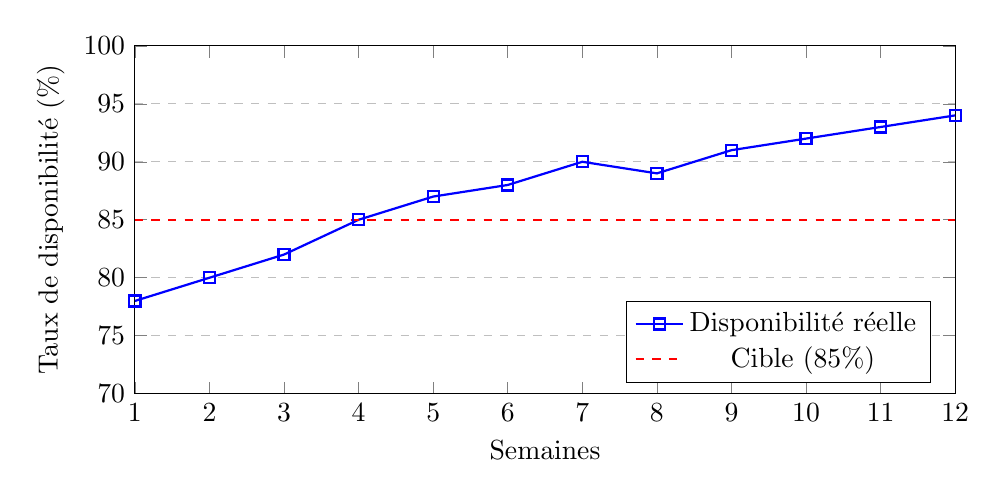
\begin{tikzpicture}
\begin{axis}[
    width=12cm,
    height=6cm,
    xlabel={Semaines},
    ylabel={Taux de disponibilité (\%)},
    ymin=70, ymax=100,
    xmin=1, xmax=12,
    xtick={1,2,3,4,5,6,7,8,9,10,11,12},
    ytick={70,75,80,85,90,95,100},
    legend pos=south east,
    ymajorgrids=true,
    grid style=dashed,
]

\addplot[
    color=blue,
    mark=square,
    thick
    ]
    coordinates {
    (1,78)(2,80)(3,82)(4,85)(5,87)(6,88)(7,90)(8,89)(9,91)(10,92)(11,93)(12,94)
    };
    \addlegendentry{Disponibilité réelle}

\addplot[
    color=red,
    mark=none,
    dashed,
    thick
    ]
    coordinates {
    (1,85)(12,85)
    };
    \addlegendentry{Cible (85\%)}

\end{axis}
\end{tikzpicture}
\caption{Exemple de suivi du taux de disponibilité des tables sur 12 semaines}
\end{figure}

\subsubsection{Mécanismes de contrôle et d'alerte}

Pour garantir la réactivité face aux dérives, des \textbf{mécanismes d'alerte automatiques} sont intégrés au système :
\begin{itemize}
  \item \textbf{Alerte de conflit} : Notification automatique lorsque deux opérations sont planifiées sur la meme table au meme moment ;
  \item \textbf{Alerte de retard} : Signal envoyé au chef d'atelier si une opération dépasse le temps prévu de plus de 20\% ;
  \item \textbf{Alerte de sous-utilisation} : Notification si une table reste inutilisée pendant plus de 2 heures consécutives en période de production ;
  \item \textbf{Rapport hebdomadaire automatique} : Génération d'un rapport récapitulatif des performances envoyé par email aux responsables.
\end{itemize}

Ces alertes permettent une \textbf{intervention rapide} et évitent l'accumulation de dysfonctionnements.

\subsubsection{Standardisation des procédures}

La pérennisation des améliorations passe par la \textbf{formalisation et la standardisation} des nouvelles pratiques. Cela inclut :
\begin{itemize}
  \item \textbf{Rédaction de procédures opératoires standardisées (SOP)} décrivant l'utilisation de l'algorithme de gestion des tables ;
  \item \textbf{Formation du personnel} a l'utilisation de l'outil et aux nouvelles méthodes de planification ;
  \item \textbf{Documentation des bonnes pratiques} : création d'un guide utilisateur illustré, accessible a tous les opérateurs ;
  \item \textbf{Audits réguliers} : vérification trimestrielle du respect des procédures et de l'utilisation effective de l'outil.
\end{itemize}

\subsubsection{Amélioration continue}

La phase de contrôle ne se limite pas a maintenir les acquis, elle s'inscrit dans une logique d'\textbf{amélioration continue} (Kaizen). Des \textbf{réunions d'amélioration} sont organisées mensuellement avec l'équipe de production pour :
\begin{itemize}
  \item Analyser les résultats des indicateurs de performance ;
  \item Identifier les nouvelles opportunités d'optimisation ;
  \item Recueillir les retours d'expérience des opérateurs ;
  \item Ajuster l'algorithme ou les procédures en fonction des besoins terrain.
\end{itemize}

Un \textbf{cycle PDCA} (Plan-Do-Check-Act) est ainsi instauré pour garantir une dynamique d'amélioration permanente.

\subsubsection{Conclusion de la phase Contrôler}

La phase de contrôle assure la \textbf{pérennité des gains} obtenus grace a l'algorithme de gestion des tables de matelassage. En combinant suivi des indicateurs, mécanismes d'alerte, standardisation des pratiques et amélioration continue, cette phase garantit que les bénéfices de la transformation digitale se maintiennent dans le temps et continuent de s'améliorer.

Cette démarche DMAIC complète, de la définition du problème jusqu'au contrôle des solutions, constitue le socle méthodologique de la transformation Lean 4.0 de l'atelier de coupe, préparant ainsi le terrain pour les développements techniques détaillés dans les chapitres suivants.
